\documentclass[conference]{IEEEtran}
\IEEEoverridecommandlockouts
% The preceding line is only needed to identify funding in the first footnote. If that is unneeded, please comment it out.
%Template version as of 6/27/2024

\usepackage{cite}
\usepackage{amsmath,amssymb,amsfonts}
\usepackage{algorithmic}
\usepackage{graphicx}
\usepackage{textcomp}
\usepackage{xcolor}
\usepackage{float}
\sloppy
\def\BibTeX{{\rm B\kern-.05em{\sc i\kern-.025em b}\kern-.08em
    T\kern-.1667em\lower.7ex\hbox{E}\kern-.125emX}}
\begin{document}

\title{Analysis of the influence of soil characteristics in the risk of landslides using a data mining approach\\}

\author{
    \IEEEauthorblockN{
        Muhammad Raihan\IEEEauthorrefmark{1},
        An Naura Erwana Dwi Putri\IEEEauthorrefmark{1},
        Amalia Diah Ramadani\IEEEauthorrefmark{1},
        \\Resky Auliyah Kartini Askin\IEEEauthorrefmark{1},
        Michael Gabriel Bida\IEEEauthorrefmark{1}
    }
    \IEEEauthorblockA{\IEEEauthorrefmark{1}Hasanuddin University, Makassar, Indonesia \\
    reskyauliyah@unhas.ac.id, annaura@unhas.ac.id, amalia.ramadani@unhas.ac.id, \\raihan.m@unhas.ac.id, michael.bida@unhas.ac.id}
}


\maketitle

\begin{abstract}
Landslides are common natural disasters in hilly regions, particularly in Indonesia, often causing significant economic and social damage. While rainfall is widely recognized as a key trigger, soil physical properties such as texture, bulk density, pH, and organic matter content also play a critical role in landslide susceptibility. This study investigates the influence of soil characteristics on landslide risk and develops a predictive model using data mining, enhanced by an interactive dashboard visualization. Two primary datasets, HWSD and WLD, were integrated for analysis. Statistical tests \textit{t}-test and Mann–Whitney \textit{U} and the XGBoost algorithm were applied. Results show that subsoil properties contribute more to landslide risk than topsoil AUC 0.7205 vs. 0.6984, with the combined model yielding the best performance AUC 0.85. These findings highlight the importance of subsoil properties in slope stability and landslide prediction, offering valuable insights for improving early warning and mitigation systems.
\end{abstract}


\section{Introduction}

Landslides are one of the deadliest natural disasters in the world, especially in tropical and mountainous regions such as South Asia and Southeast Asia. According to data from the Centre for Research on the Epidemiology of Disasters (CRED), landslides caused more than 55,000 deaths globally between 2004 and 2016, with more than 75\% of these events occurring in Asia~\cite{intro01}. 
The main triggers in these regions include extreme rainfall, seismic activity, and vulnerable geological conditions. 

Although those factor is often considered the dominant trigger as noted in~\cite{intro02}, recent studies highlight the critical role of soil physical properties such as texture, permeability, and density in influencing slope stability~\cite{intro03}. 
However, most existing early warning systems still rely heavily on meteorological and topographical data, while pedological information is often overlooked.

This study focuses on two main soil layers, namely topsoil (upper layer) and subsoil (lower layer), both of which have different characteristics and hydrological functions in slope failure mechanisms. Topsoil is rich in organic matter and more porous, functioning as the first layer to receive and infiltrate rainwater. In contrast, subsoil tends to be denser, has a higher clay content, and lower permeability. 
During periods of intense rainfall, water that seeps through the topsoil can accumulate above the subsoil layer, causing a significant increase in pore water pressure. This increase in pressure reduces the internal shear strength of the soil, which is a key factor in triggering landslides.

To analyze the relationship between soil characteristics in both topsoil and subsoil layers in landslide and non-landslide areas, this study applied a two stage approach. The first stage was an inferential statistical analysis to test the significance of differences in soil properties between landslide and non-landslide locations. 
For this purpose, an independent t-test was applied to normally distributed data and a non-parametric Mann-Whitney U test was applied to data that did not meet the assumption of normality. These two tests served to quantitatively validate whether a soil feature had a significant difference between the two groups, so that it could be considered a relevant distinguishing factor. 

The second stage is predictive modeling using machine learning algorithms. 
Based on statistically significant features, an Extreme Gradient Boosting (XGBoost) model was developed to predict the probability of landslide risk. This algorithm was chosen for its proven superior performance, ability to model complex feature interactions, and resistance to overfitting.

However, one of the main challenges in this modeling is the class imbalance in the dataset, where the amount of non-landslide data is much greater than the landslide data. To overcome this problem, an oversampling technique using the Synthetic Minority Over-sampling Technique (SMOTE) was applied. 
Next, the XGBoost model was trained using a balanced dataset, with hyperparameter optimization performed through Bayesian Optimization to achieve maximum performance. Model evaluation was carried out using a Stratified K-Fold Cross-Validation scheme to ensure robustness, with key performance metrics including F1-score and Receiver Operating Characteristic Area Under the Curve (ROC-AUC).
Through this approach, the study aims to develop a landslide risk prediction model based on soil properties that is not only accurate but also provides an overview of the contribution of pedological features. The results of this study are expected to form the basis for future research to integrate soil data with other key triggers, such as meteorological and topographical data, in order to improve early warning systems in the future.

\section{Methodlogy}

\subsection{Study Area}
This study is based on data from 13 countries across five continents: Australia, Brazil, China, Costa Rica, Ecuador, Italy, Mexico, New Zealand, Norway, Pakistan, South Africa, Taiwan, and Vietnam. The selection of these nations was guided by two primary criteria: a significant diversity of soil types , as indexed by the Harmonized World Soil Database (HWSD) and a high frequency of recorded landslides between 2006 and 2017, as documented in NASA's Global Landslide Catalog (GLC).
\begin{figure}[htbp]
    \centerline{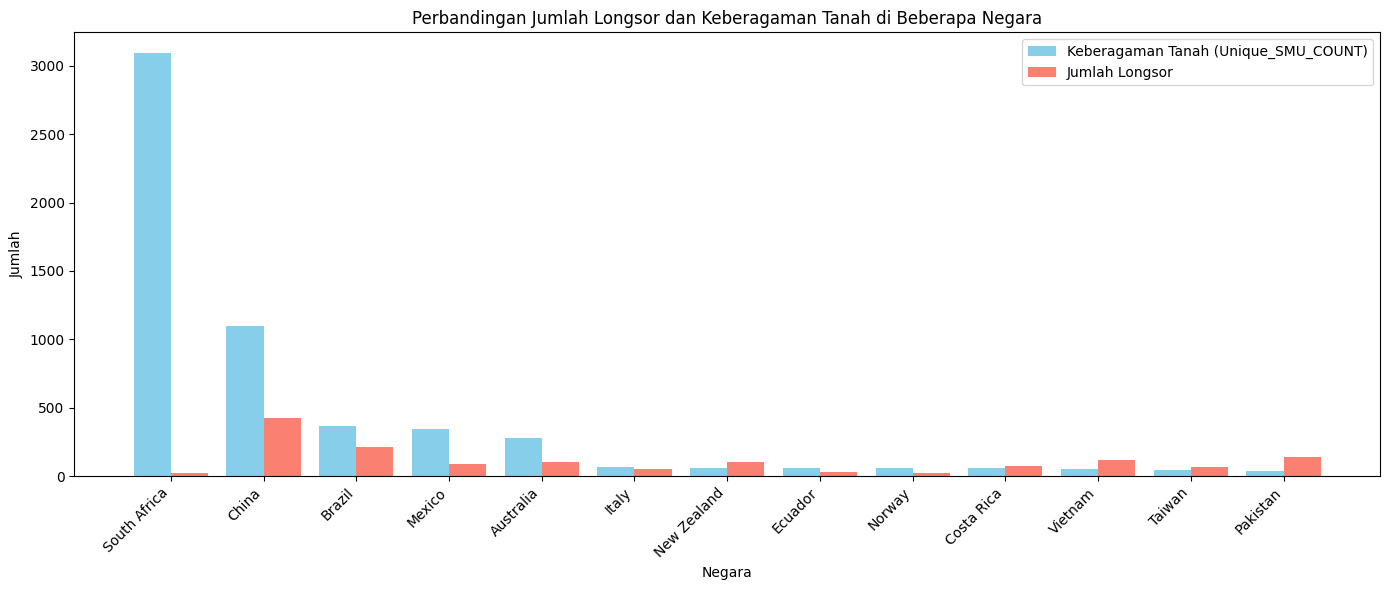
\includegraphics[width=\linewidth]{fig1.png}}
    \caption{Landslide events vs. unique soil characteristics.}
    \label{fig:landslide-soil-distribution}
\end{figure}
Figure~\ref{fig:landslide-soil-distribution} illustrates the distribution of landslide events and soil diversity (represented by the count of unique Soil Mapping Units) for the selected countries. For most nations, a general correspondence is observed between the two metrics. South Africa, however, presents a notable exception, exhibiting exceptionally high soil diversity relative to its number of recorded landslides. This broad geographical scope inherently introduces significant variations in other key landslide-triggering factors, such as climate patterns (ranging from tropical to temperate), topography (from steep mountainous terrain to gentle hills), and land cover, which is essential for developing a globally generalizable model.


\subsection{Datasets}
This study integrates data from three primary sources. Soil characteristics were derived from the Harmonized World Soil Database (HWSD), a 30 arc-second raster database providing presents soil information collected from various regional and national sources, including the European Soil Database (ESDB), the 1:1,000,000 scale Soil Map of China, and various legacy soil maps from Food and Agriculture Organization (FAO). Data from these different sources were harmonized using standard procedures. The database consists of a raster image that is linked to the attribute database through a unique code of the soil mapping unit. For each mapping unit, the database provides information on the composition of the soil types present in it (dominant soils and accompanying soils). It also contains quantitative data on soil physical and chemical properties for two depth layers, namely topsoil (0-30 cm) and subsoil (30-100 cm). These attributes include organic carbon content, pH, water holding capacity, soil depth, cation exchange capacity, clay fraction, salinity, and soil texture. Table 1 describes the classification of data sources and their data types and table 2 describes general information on the soil mapping unit composition.

\begin{table}[H]
\caption{Data Sources and Outputs in the Harmonized World Soil Database}
\centering
\begin{tabular}{|c|l|l|l|} 
\hline
\textbf{No.} & \multicolumn{1}{|c|}{\textbf{Data Source}} & \multicolumn{1}{|c|}{\textbf{Format}} & \multicolumn{1}{|c|}{\textbf{Output}} \\
\cline{2-4} 
\textbf{} & \textbf{\textit{Database Name}} & \textbf{\textit{Data Type}} & \textbf{\textit{Resolution/Quantity}} \\
\hline
1 & ESDB & Geo. DB & Raster $\sim$1 km \\
\hline
2 & Soil Map China & Digital Map & Raster $\sim$1 km \\
\hline
3 & SOTER (World Soils and Terrain Database) (SOTWIS: SOTER World Information System) & Soil & Raster $\sim$1 km \\
\hline
4 & Soil Map World & Digital Map & Raster $\sim$1 km \\
\hline
5 & Soil Profile DB & Profile Data & 9607 profiles \\
\hline
\multicolumn{4}{l}{$^{\mathrm{a}}$ESDB: European Soil Database. Geo. DB: Geographic Database.} \\
\multicolumn{4}{l}{$^{\mathrm{b}}$Soil Map of China; SOTER: World Soils and Terrain Database.} \\
\multicolumn{4}{l}{$^{\mathrm{c}}$Soil Profile DB: Soil Profile Database.} \\
\multicolumn{4}{l}{$^{\mathrm{d}}$Input Scale/Resolution for raster data (1:1M or 1:10M).} \\
\multicolumn{4}{l}{$^{\mathrm{e}}$Input Scale/Resolution for SOTER databases (1:2.5M – 5M).}
\end{tabular}
\label{tab:hwsd_sources_compact}
\end{table}

Historical landslide event data were obtained from the NASA Global Landslide Catalog (GLC), from which we extracted all documented rainfall-triggered landslides occurring between 2006 and 2017. Finally, all data were geographically contextualized using the Natural Earth “Admin 0 – Countries” vector dataset (1:10m scale) to define the national administrative boundaries for the study area.


\subsection{Method}

The methodology adopted in this study is systematically illustrated in Figure~\ref{fig:research-workflow}. The research commenced with an extensive literature review on soil characteristics and landslide occurrences to gather relevant data. Subsequently, three distinct datasets were compiled and integrated.

\begin{figure}[htbp]
    \centerline{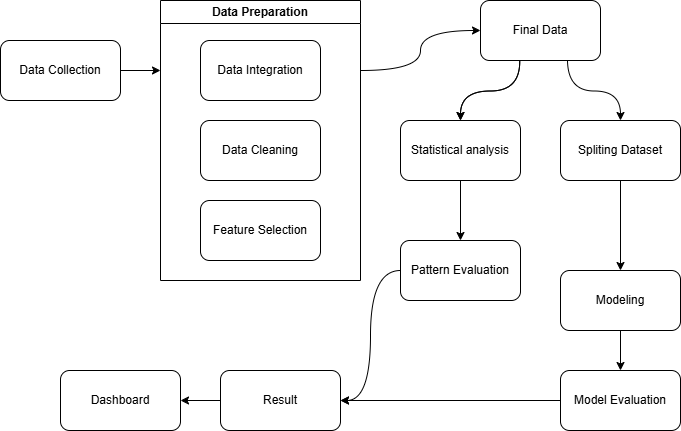
\includegraphics[width=\linewidth]{fig2.png}}
    \caption{research workflow}
    \label{fig:research-workflow}
\end{figure}
This integration process was guided by two primary references: the HWSD Technical Report and Instructions and a technical note by D.G. Rossiter, Processing the Harmonized World Soil Database (Version 1.2) in R. A detailed flowchart of the data integration procedure is presented in Figure~\ref{fig:data-integration-workflow}. From the study area, a total of 2,210 landslide and non-landslide data, each corresponding to different soil characteristics, were identified.

\begin{table}[H]
\caption{Field Availability in Soil Databases (Simplified)}
\centering
\begin{tabular}{|p{2cm}|p{2.8cm}|c|}
\hline
\textbf{Field} & \textbf{Description} & \textbf{DSMW (Digital Soil Map of the World)} \\
\hline
\multicolumn{3}{|l|}{\textbf{General}} \\
\hline
ID & Database ID & $\surd$ \\
MU\_GLOBAL & Global Unit ID & $\surd$ \\
COVERAGE & Coverage & $\surd$ \\
ISSOIL & Soil indicator & $\surd$ \\
SHARE & Share in Unit & $\surd$ \\
SU\_SYMBOL & Symbol & $\surd$ \\
\hline
\multicolumn{3}{|l|}{\textbf{Phases and Additional}} \\
\hline
PHASE1 & Phase 1 & $\surd$ \\
ROOTS & Root obstacles &  \\
AWC\_CLASS & AWC Class & $\surd$ \\
\hline
\end{tabular}
\label{tab:soil_field_availability_small}
\end{table}

\begin{figure}[htbp]
    \centerline{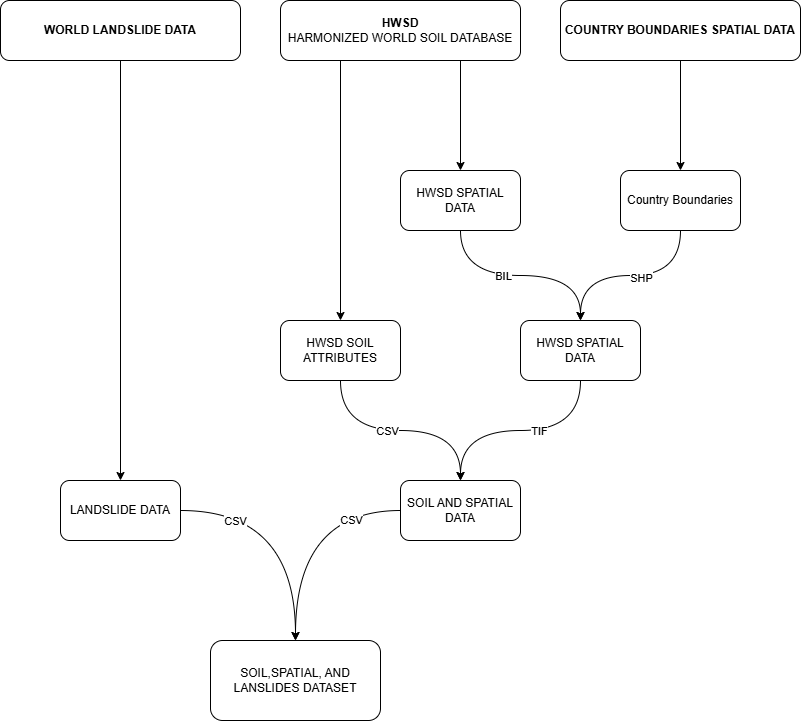
\includegraphics[width=\linewidth]{fig3.png}}
    \caption{Data Integration Workflow}
    \label{fig:data-integration-workflow}
\end{figure}

Following data integration, a comprehensive data preprocessing phase was conducted. This began with data cleaning, in which missing values were imputed using the median of their respective columns. Subsequently, outlier handling was performed using the Interquartile Range (IQR) method\cite{mthd01}. This analysis revealed numerous outliers across most feature columns; these were also imputed using the column-specific median in order to maintain data integrity.
The next stage focused on feature selection. Features were removed based on three criteria: identifier columns (as listed in Table~\ref{tab:soil_field_availability_small}), columns containing only a single unique value, and those with low feature importance scores method. A machine learning-based approach using the XGBoost algorithm was employed to assess the importance of each remaining feature\cite{mthd02}. The results of this analysis, visualized in Figure~\ref{fig:feature-importance}, identified two features—\texttt{AWC\_CLASS} and \texttt{S\_CASO4}—with an importance score of zero. Consequently, these non-contributory features were removed from the dataset.

The final preprocessing step was data transformation. Label encoding was applied to the categorical feature 'COUNTRY'. This method was selected for its suitability with tree-based models, which are invariant to the ordinal relationships that might be artificially introduced by other encoding techniques\cite{mthd03}. 
\begin{figure}[htbp]
    \centerline{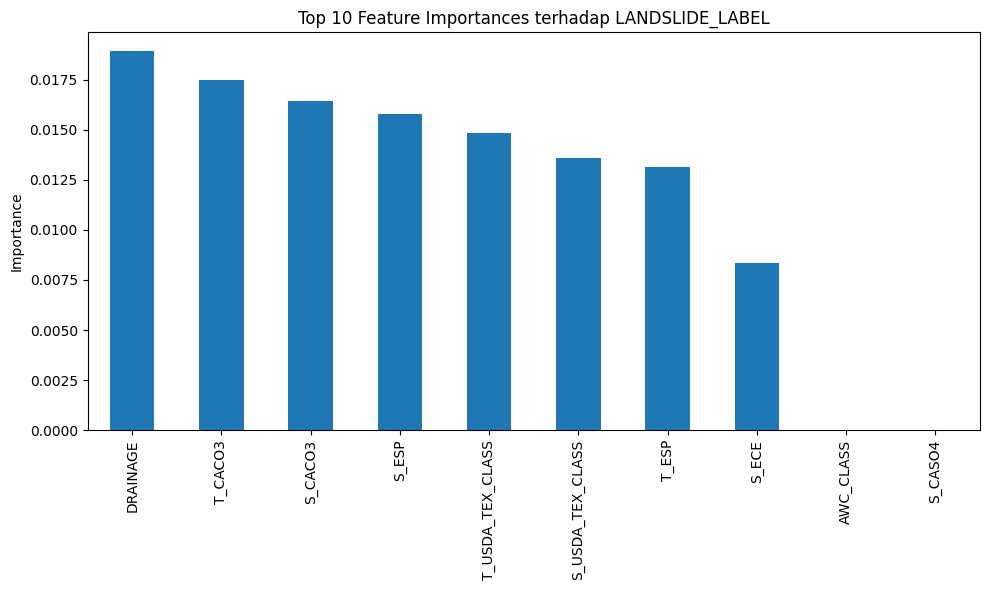
\includegraphics[width=\linewidth]{fig4.png}}
    \caption{Feature Importance Analysis}
    \label{fig:feature-importance}
\end{figure}
This study employs two primary analytical approaches: statistical analysis and machine learning modeling.

\subsubsection{statistical analysis}
Statistical analysis was conducted to identify significant differences in soil characteristics between two predefined groups: locations where landslides occurred (labeled as 1) and locations where they did not (labeled as 0). To achieve this, both parametric and non-parametric hypothesis tests were applied, specifically the independent samples t-test and the Mann-Whitney U test\cite{mthd04}.

The main objective of these tests was to calculate the p-value for each soil feature. The p-value quantifies the probability that an observed difference between the groups is merely due to random chance. A lower p-value indicates a more statistically significant difference, suggesting that the corresponding soil feature is a meaningful differentiator between landslide and non-landslide conditions.

The mathematical formulation for the independent samples t-test is presented in (\ref{eq:t_test}), while the formula for the Mann-Whitney U test is detailed in (\ref{eq:mann_whitney}).

\begin{equation} \label{eq:t_test}
t = \frac{\bar{x}_1 - \bar{x}_2}{s_p \cdot \sqrt{\frac{1}{n_1} + \frac{1}{n_2}}}
\end{equation}
where $s_p$ is the pooled standard deviation, calculated as:
\begin{equation} \label{eq:sp_pooled}
s_p = \sqrt{\frac{(n_1 - 1)s_1^2 + (n_2 - 1)s_2^2}{n_1 + n_2 - 2}}
\end{equation}

For the Mann-Whitney U test, the U statistic is given by:
\begin{equation} \label{eq:mann_whitney}
U = \min(U_1, U_2)
\end{equation}
where:
\begin{align}
U_1 &= n_1n_2 + \frac{n_1(n_1 + 1)}{2} - R_1 \label{eq:U1} \\
U_2 &= n_1n_2 + \frac{n_2(n_2 + 1)}{2} - R_2 \label{eq:U2}
\end{align}
\subsubsection{machine learning modeling}
For the primary classification task, this study utilized the Extreme Gradient Boosting (XGBoost) model\cite{mthd05}. XGBoost is a highly efficient and scalable implementation of the gradient tree boosting algorithm, widely regarded as a state-of-the-art machine learning method. It employs a regularized boosting technique, which effectively mitigates overfitting and thereby enhances model accuracy and generalization performance. The selection of XGBoost was motivated by its numerous advantages, including its scalability across diverse scenarios, inherent capability to handle sparse data, low computational resource requirements, high-performance speed, and ease of implementation. The fundamental principle of the boosting algorithm is to sequentially combine the outputs of multiple weak learners---in this case, Classification and Regression Trees (CART)---to create a single, robust predictive model. The core of the algorithm aims to minimize the regularized objective function, as formulated in Equation~\ref{eq:objective_function}. This function is composed of two main parts: a loss function and a regularization term. The loss function measures the discrepancy between the actual target ($y_i$) and the prediction ($\hat{y}_i$). The second component, the regularization term detailed in (\ref{eq:regularization_term}), penalizes the complexity of the model to avoid overfitting. The overall algorithmic process is described by (\ref{eq:objective_function}) through (\ref{eq:simplified_objective_function_t}).
% Equation (3) - Objective Function
\begin{equation} \label{eq:objective_function}
L(\Phi) = \sum_i l(\hat{y}_i, y_i) + \sum_k \Omega(f_k)
\end{equation}

% Equation (4) - Regularization Term
\begin{equation} \label{eq:regularization_term}
\Omega(f) = \gamma T + \frac{1}{2} \lambda \|w\|^2
\end{equation}
where:
\begin{itemize}
    \item $T$: the number of leaves in the tree;
    \item $w$: the score of each leaf;
    \item $\gamma, \lambda$: the regularization degrees.
\end{itemize}

% Equation (5) - Objective Function at iteration t
\begin{equation} \label{eq:objective_function_t}
L^{(t)}(\Phi) = \sum_{i=1}^n l(y_i, \hat{y}_i^{(t-1)} + f_t(x_i)) + \Omega(f_t)
\end{equation}

In order to speed up the optimization process, second order Taylor expansion is applied to the objective. After removing the constant terms, a simplified objective function at step $t$ is given in (\ref{eq:simplified_objective_function_t}).

% Equation (6) - Simplified Objective Function at iteration t
\begin{equation} \label{eq:simplified_objective_function_t}
\tilde{L}^{(t)} = \sum_{i=1}^n \left[ g_i f_t(x_i) + \frac{1}{2} h_i f_t^2(x_i) \right] + \Omega(f_t)
\end{equation}
where:
\begin{align} \label{eq:g_h_definitions}
g_i &= \partial_{\hat{y}_i^{(t-1)}} l(y_i, \hat{y}_i^{(t-1)}) \\
h_i &= \partial_{\hat{y}_i^{(t-1)}}^2 l(y_i, \hat{y}_i^{(t-1)})
\end{align}
The preprocessed dataset was partitioned for training and validation using a 5-fold StratifiedKFold cross-validation scheme\cite{mthd06}. This approach effectively splits the data into an 80\% training set and a 20\% testing set during each fold, while critically preserving the original class distribution (landslide vs. non-landslide) across all folds. This stratification is essential for ensuring reliable model evaluation on an imbalanced dataset. To address the class imbalance issue, the SMOTE (Synthetic Minority Over-sampling Technique) was applied to the training data to synthetically oversample the minority (landslide) class\cite{mthd07}.

The XGBoost classification algorithm was used and evaluated in this study. To enhance the models' sensitivity to the positive class (landslide), a class weight adjustment mechanism was integrated into the training process. Hyperparameter optimization was conducted efficiently using Bayesian Optimization implemented via BayesSearchCV\cite{mthd08}, facilitating an effective search for the optimal parameter combination within a predefined search space.

Model performance was assessed using a suite of standard classification metrics. The Confusion Matrix served as the foundation for performance analysis\cite{mthd09}, categorizing predictions into four distinct outcomes: True Positives (TP), False Positives (FP), True Negatives (TN), and False Negatives (FN), as illustrated in Figure 5.

The primary evaluation metric for this study was the F1-Score, which is the harmonic mean of precision and recall, providing a balanced measure of performance on imbalanced data. Furthermore, the classification threshold was tuned to achieve a desired level of recall. The Receiver Operating Characteristic (ROC) curve was also utilized to visualize the discriminative ability of the models across various thresholds. This curve is generated by plotting the True Positive Rate (TPR) against the False Positive Rate (FPR), where the area under the curve (AUC-ROC) provides an aggregate measure of performance across all classification thresholds.
\begin{figure}[H]
    \centerline{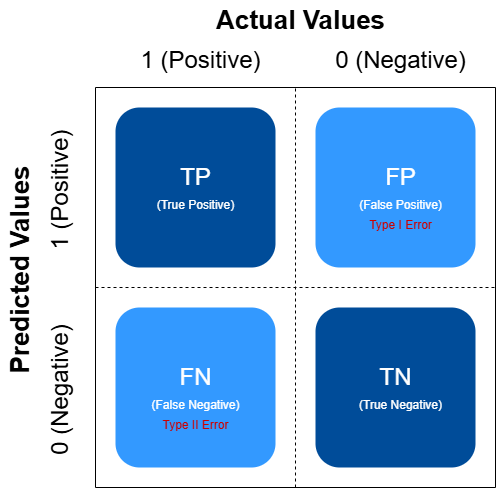
\includegraphics[width=\linewidth]{fig5.png}}
    \caption{Metrics for evaluating classification performance.}
    \label{fig}
\end{figure}

The sensitivity (True positive or Recall) tells the proportion of positive class (landslides locations) that are correctly classified as landslides (\ref{eq:sensitivity}). In contrast, the specificity (True Negative Rate) tells the proportion of negative class (non-landslides locations) that are correctly classified as non-landslides (\ref{eq:specificity}). Between sensitivity and specificity lies False Negative Rate (FNR), which signifies the proportion of landslide points wrongly classified as landslides (\ref{eq:FNR}). The False Positive Rate (FPR) tells the proportion of non-landslides incorrectly classified as non-landslides (\ref{eq:FPR}).

\begin{equation} \label{eq:sensitivity}
\text{sensitivity} = \frac{TP}{TP + FN}
\end{equation}

\begin{equation} \label{eq:specificity}
\text{specificity} = \frac{TN}{TN + FP}
\end{equation}

\begin{equation} \label{eq:FNR}
\text{FNR} = \frac{FN}{TP + FN}
\end{equation}

\begin{equation} \label{eq:FPR}
\text{FPR} = \frac{FP}{TN + FP} = 1 - \text{specificity}
\end{equation}





\section{Result}
By comparing the data distribution of soil characteristics in both the landslide and no landslide groups, as illustrated in Figure~\ref{fig:Violin-plot}, it can be observed that the two groups exhibit differences in distribution, although not always significant. Taking the \textit{S\_CLAY} feature as an example—which represents the clay content in the subgrade—it is evident that the no landslide group shows a data concentration between 20 and 40, with a median value tending to lie below 40. In contrast, the landslide group exhibits a concentration between 30 and 60, with a higher median than the no landslide group. This suggests that landslide-prone areas tend to have higher clay content compared to non-landslide areas.

To support this observation, a statistical analysis was conducted to calculate the \textit{p}-value using Equations~\ref{eq:t_test} or \ref{eq:mann_whitney} (the formula used depends on the data distribution, if the data distribution is normal then use t-test and u whitney-u otherwise). The \texttt{S\_CLAY} feature yielded a \textit{p}-value of $6.38 \times 10^{-5}$ (or 0.0000638), which is much smaller than the significance threshold of 0.05. This indicates a statistically significant difference between the two groups.

\begin{figure}[htbp]
    \centerline{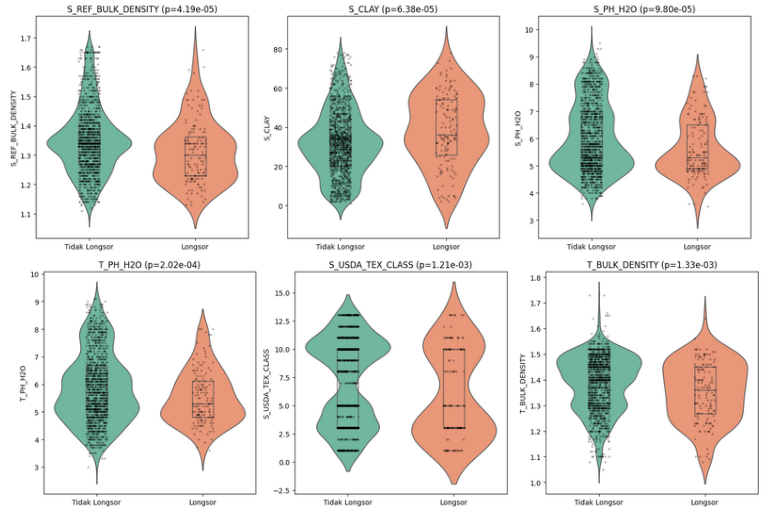
\includegraphics[width=\linewidth]{fig6.png}}
    \caption{Violin Plot of Topsoil vs Subsoil.}
    \label{fig:Violin-plot}
\end{figure}

To evaluate the relative predictive contribution of different soil layers, separate classification analyses were conducted for topsoil and subsoil features. The discriminative performance of these two feature sets was then evaluated using ROC (Receiver Operating Characteristic) curves and AUC (Area Under the Curve) values. The results, as shown in Figure~\ref{fig:sub-top}, indicate that the model trained using the subsoil features achieved slightly superior predictive performance with an AUC value of 0.7205, compared to the model using the topsoil features with an AUC of 0.6984.

To further investigate the performance difference between the two soil layers, a feature importance analysis was conducted, as illustrated in Figure~\ref{fig:feature-importance-top-sub}. In the topsoil layer, the most influential features were primarily related to soil chemical properties, including Electrical Conductivity (T\_ECE), Calcium Carbonate (T\_CACO3), Total Exchangeable Bases (T\_TEB), and Organic Carbon (T\_OC). Meanwhile, in the subsoil layer, Calcium Carbonate (S\_CACO3) and Electrical Conductivity (S\_ECE) were the top contributors, followed by texture classification (S\_USDA\_TEX\_CLASS) and Total Exchangeable Bases (S\_TEB). These findings highlight that subsoil characteristics—particularly chemical and textural properties—play a more critical role in predicting landslide susceptibility.

Collectively, these findings suggest that while both soil layers contribute valuable information, subsoil characteristics—particularly those related to chemical composition and texture classification—exhibit greater predictive power in landslide risk modeling compared to topsoil features.

\begin{figure}[htbp]
    \centerline{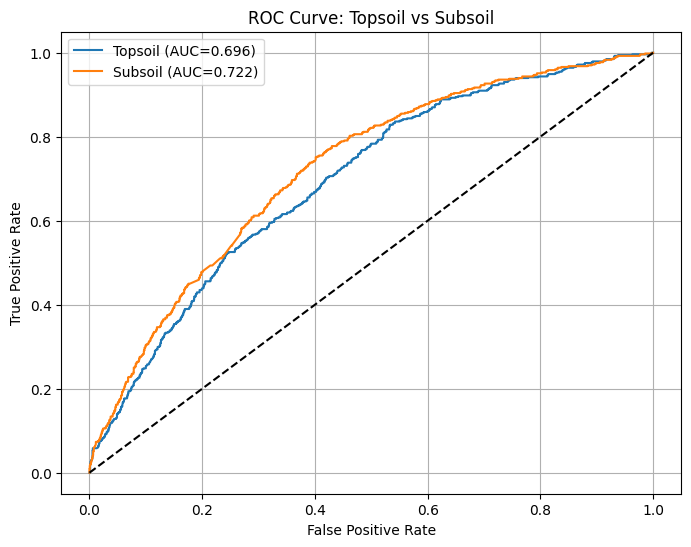
\includegraphics[width=\linewidth]{fig7.png}}
    \caption{ROC-AUC of Topsoil and Subsoil Layers.}
    \label{fig:sub-top}
\end{figure}
\begin{figure}[htbp]
    \centerline{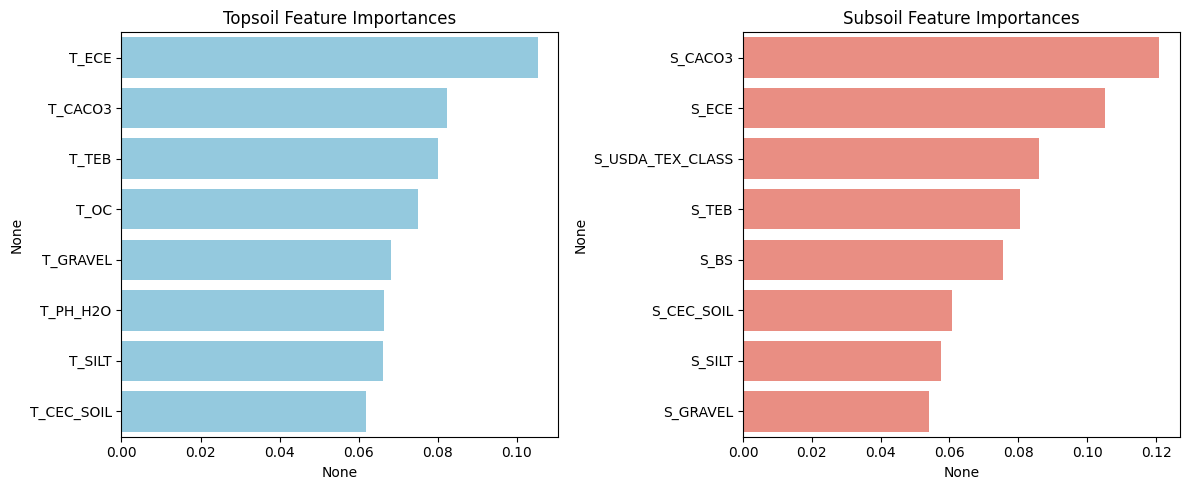
\includegraphics[width=\linewidth]{fig8.png}}
    \caption{Feature importance of Topsoil and Subsoil Layers.}
    \label{fig:feature-importance-top-sub}
\end{figure}

As a final step, a comprehensive model was trained by combining features from the topsoil and subsoil layers to evaluate their synergistic effects. The evaluation results of this combined model, visualized in the ROC curve in Figure~\ref{fig:all-layers}, show a significant improvement in performance, achieving an AUC value of 0.85. This value far surpasses the performance of the model using only one of the layers separately.

This substantial improvement confirms that although the subsoil characteristics have a slightly more dominant predictive power, information from the topsoil also makes an essential complementary contribution. Thus, it can be concluded that holistic soil profile analysis---considering the interaction between both layers---is the most effective approach for landslide risk modeling with the highest accuracy.

\begin{figure}[htbp]
    \centerline{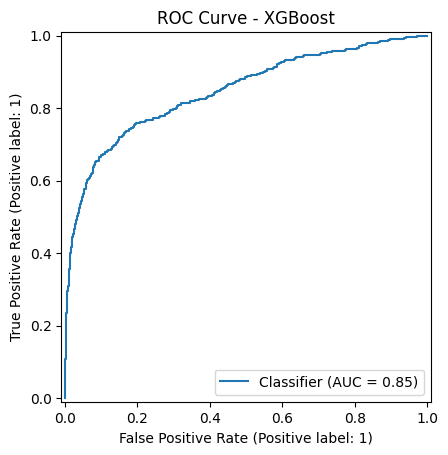
\includegraphics[width=\linewidth]{fig9.png}}
    \caption{ROC-AUC curve for all layers.}
    \label{fig:all-layers}
\end{figure}
\begin{figure}[htbp]
    \centerline{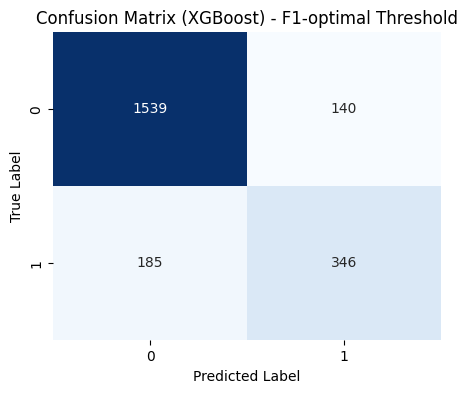
\includegraphics[width=\linewidth]{fig10.png}}
    \caption{Confussion matrix.}
    \label{fig:confusion-matrix}
\end{figure}

In Figure~\ref{fig:confusion-matrix} the confusion matrix shows that out of a total of 531 actual landslide events (class 1), the model correctly identified 346 of them (True Positive), while 185 events were missed (False Negative). For the non-landslide class (class 0), the model demonstrated strong performance with 1539 correct predictions (True Negative) and only 140 incorrect predictions (False Positive).

This is reflected in the classification report, where the model achieved a recall of 0.65 and a precision of 0.71 for the landslide class, resulting in an F1-score of 0.68. The overall accuracy of the model reached 85.29\%, indicating generally reliable predictive capability. With a weighted average F1-score of 0.85, the model demonstrates an effective balance between precision and recall across the dataset, validating the success of the optimization strategy on imbalanced data.

\section{Discussion}

A statistical significance test was conducted to examine the differences in soil characteristics between landslide and non-landslide groups, as illustrated in the violin plots (Fig. \textit{ref}). The aim of this analysis was to verify whether there were significant distinctions in soil attributes between the two groups. For this purpose, both the \textit{t}-test and Mann–Whitney \textit{U} test were employed. The use of such statistical tests follows similar methodologies adopted in prior studies. For instance, \cite{b1} applied the Mann–Whitney \textit{U} test to compare soil properties such as clay content, bulk density, and pH between landslide-affected and unaffected areas in the Three Gorges Reservoir, while \cite{b2} employed the Mann–Whitney \textit{U} test for non-normally distributed data and the \textit{t}-test for normally distributed data to evaluate differences in soil porosity, organic content, and texture in landslide-prone areas of the Himalayas.

The results depicted in the violin plots reveal several soil characteristics exhibiting significant differences, as indicated by p-values less than 0.05. Notably, variables such as \texttt{s\_clay} and \texttt{s\_ref\_bulk density} demonstrate statistically significant differences between the landslide and non-landslide groups. These findings are consistent with the observations reported by \cite{b3}, who stated that thick clay layers with low bulk density, due to their loose structure, render the soil more susceptible to landslides.

Performance indicators such as the Receiver Operating Characteristic (ROC), Area Under the Curve (AUC), and evaluation matrices (Fig. \textit{ref}) were used to validate the predictive capability of the XGBoost algorithm. These indicators follow evaluation standards similar to those employed by \cite{b4}, who used ROC-AUC to assess landslide susceptibility mapping using XGBoost. Furthermore, the model separates the analysis between topsoil and subsoil layers, following the approach of \cite{b5}, who investigated how different soil layers influence mass movement events.

As shown in Fig. \textit{ref}, the comparison of XGBoost model performance between the two soil layers yielded an AUC of 0.6984 for topsoil and 0.7205 for subsoil. Although the difference is not statistically significant, the subsoil layer exhibited slightly superior predictive performance. This aligns with findings reported by \cite{b6}, who noted that subsoil layers exhibit more stable properties—such as organic content and texture—over time, particularly after landslide events, thereby making them more suitable for long-term landslide analysis.

An additional model evaluation was conducted by integrating both topsoil and subsoil data, as shown in Fig. \textit{ref}, resulting in a significant increase in AUC to 0.85. This suggests that combining both soil layers enhances model performance, with subsoil data contributing more strongly to the prediction. Landslide analysis using data mining approaches has proven to be a valuable tool for spatial planning and land management. However, it remains a challenge to achieve high model prediction performance using soil properties alone. As demonstrated by \cite{b7}, incorporating other environmental factors such as rainfall and slope gradients can significantly improve model performance, achieving an AUC of 0.89, even though the geographical context differs.


\section{Conclusion}

The results of this study demonstrate that stratifying soil characteristics by depth—topsoil and subsoil—offers a more nuanced understanding of their respective contributions to landslide susceptibility. The XGBoost model trained on subsoil features outperformed the topsoil-based model (AUC = 0.7205 vs. 0.6984), while the combined model yielded the highest performance (AUC = 0.85; F1-score = 0.68). These findings confirm that incorporating a holistic soil profile enhances predictive accuracy.

The application of SMOTE to address class imbalance, coupled with Bayesian Optimization for hyperparameter tuning, proved effective in increasing the model’s sensitivity to landslide events. Nonetheless, limitations persist in the generalizability of the optimized parameters, as the best-performing configuration in one cross-validation fold may not consistently perform well across others.

Feature importance analysis indicated that subsoil chemical properties—such as calcium carbonate content and electrical conductivity—play a pivotal role in landslide prediction. Additionally, soil textural attributes and cation exchange capacity further contributed to improved model performance, underscoring the complex interplay between physical and chemical soil factors in landslide initiation.

This study advances the development of soil-based early warning systems and provides valuable insights into key indicators of landslide risk. Future research should consider incorporating additional environmental variables, such as rainfall intensity, slope gradient, and land cover, to construct more comprehensive and spatially robust predictive models.

\section*{Acknowledgment}

The preferred spelling of the word ``acknowledgment'' in America is without 
an ``e'' after the ``g''. Avoid the stilted expression ``one of us (R. B. 
G.) thanks $\ldots$''. Instead, try ``R. B. G. thanks$\ldots$''. Put sponsor 
acknowledgments in the unnumbered footnote on the first page.

\section*{References}

Please number citations consecutively within brackets \cite{b1}. The 
sentence punctuation follows the bracket \cite{b2}. Refer simply to the reference 
number, as in \cite{b3}---do not use ``Ref. \cite{b3}'' or ``reference \cite{b3}'' except at 
the beginning of a sentence: ``Reference \cite{b3} was the first $\ldots$''

Number footnotes separately in superscripts. Place the actual footnote at 
the bottom of the column in which it was cited. Do not put footnotes in the 
abstract or reference list. Use letters for table footnotes.

Unless there are six authors or more give all authors' names; do not use 
``et al.''. Papers that have not been published, even if they have been 
submitted for publication, should be cited as ``unpublished'' \cite{b4}. Papers 
that have been accepted for publication should be cited as ``in press'' \cite{b5}. 
Capitalize only the first word in a paper title, except for proper nouns and 
element symbols.

For papers published in translation journals, please give the English 
citation first, followed by the original foreign-language citation \cite{b6}.

\begin{thebibliography}{00} 
\bibitem{b1} M. J. Froude and D. N. Petley, "Global fatal landslide occurrence from 2004 to 2016," *Natural Hazards and Earth System Sciences*, vol. 18, pp. 2161–2181, 2018, doi: 10.5194/nhess-18-2161-2018.
\bibitem{b2} W. Budianta \emph{et al.}, "The effect of clay-soil on landslide: Case study from Central Java, Indonesia," \emph{IOP Conference Series: Earth and Environmental Science}, vol. 1091, no. 1, p. 012012, 2022, doi:10.1088/1755-1315/1091/1/012012.
\bibitem{b3} Petley, D. (2012). Global patterns of loss of life from landslides. Geology, 40(10), 927–930. https://doi.org/10.1130/G33217.1
\bibitem{b4} Froude, M. J., \& Petley, D. N. (2018). Global fatal landslide occurrence from 2004 to 2016. Natural Hazards and Earth System Sciences, 18(8), 2161–2181. https://doi.org/10.5194/nhess-18-2161-2018
\bibitem{b5} Bergstra, J., \& Bengio, Y. (2012). Random Search for Hyper-Parameter Optimization. Journal of Machine Learning Research, 13(1), 281–305. http://www.jmlr.org/papers/volume13/bergstra12a/bergstra12a.pdf
\bibitem{b1} Z. Guo, L. Chen, K. Yin, D. P. Shrestha, and L. Zhang, “Quantitative risk assessment of slow-moving landslides from the viewpoint of decision-making: A case study of the Three Gorges Reservoir in China,” Engineering Geology, vol. 273, Art. no. 105667, Aug. 2020.
\bibitem{b2} Z. Habib, A. Kumar, R. A. Mir, I. M. Bhat, W. Qader, and R. K. Mallik, “Geotechnical analysis and landslide susceptibility of overburden slope material in the Jammu and Kashmir, Western Himalaya,” Geosystems and Geoenvironment, in press, Art. no. 100413, May 2025. DOI: 10.1016/j.geogeo.2025.100413
\bibitem{b3} J. Sartohadi, N. A. H. J. Pulungan, M. Nurudin, and W. Wahyudi, “The ecological perspective of landslides at soils with high clay content in the Middle Bogowonto Watershed, Central Java, Indonesia,” Applied and Environmental Soil Science, vol. 2018, Art. ID 2648185, May 2018. DOI: 10.1155/2018/2648185
\bibitem{b4} S. Badola, V. N. Mishra, and S. Parkash, "Landslide susceptibility mapping using XGBoost machine learning method," in Proc. 2023 Int. Conf. Machine Intelligence for GeoAnalytics and Remote Sensing (MIGARS), Hyderabad, India, 2023, pp. 1–4, doi: 10.1109/MIGARS57353.2023.10064496.
\bibitem{b5} A. Parasyris, L. Stankovic, and V. Stankovic, "A Machine Learning-Driven Approach to Uncover the Influencing Factors Resulting in Soil Mass Displacement," Geosciences, vol. 14, no. 8, p. 220, Aug. 2024. doi: 10.3390/geosciences14080220.
\bibitem{b6} M. S. Kim, Y. Onda, J. K. Kim, and S. W. Kim, "Effect of topography and soil parameterisation representing soil thicknesses on shallow landslide modelling," Quaternary International, vol. 384, pp. 91–106, Oct. 2015. doi: 10.1016/j.quaint.2015.03.057.
\bibitem{b7} Y. Han and S. J. Semnani, "Important considerations in machine learning–based landslide susceptibility assessment under future climate conditions," [Journal Name Unavailable], vol. 20, pp. 475–500, 2025. Published: Aug. 3, 2024.
\end{thebibliography}

\vspace{12pt}
\color{red}
IEEE conference templates contain guidance text for composing and formatting conference papers. Please ensure that all template text is removed from your conference paper prior to submission to the conference. Failure to remove the template text from your paper may result in your paper not being published.

\end{document}
